%  Discussion.tex
% !TeX spellcheck = en_GB
% !TeX root = ReportMain.tex

\section{Discussion} \label{s:Discussion}
As has been outlined in this report so far, there are problems inherent within bushing design and multiple solutions to these problems. A full discussion and comparison will be made to determine the most accurate and reliable model for HV bushing design. Additionally, reasoning and justification for the incremental changes will outline the development of bushing and possible further improvements that could be made in design.
%BH
\subsection{Success Criteria}
In section 2 four criteria were mentioned to determine the efficacy of the design: general/intrinsic breakdown defined by the radial field, surface discharge defined by the axial field, partial discharge within the material defined by areas of high tangential field and corona discharge within air. 

Regarding general breakdown it is the largest breakdown strength of the model and so the least likely to fail. High Voltage Engineering Fundamentals has it defined as well in excess of  1MV/cm \cite{kuffel2000high}. The area of interest for this intrinsic breakdown is the line from the conductor straight to the flange, and a measurement of radial electric field.

Surface discharge is not as readily defined for typical graded designs, however a comparison can be made from shedding specifications. Shedding increases the effective creepage length of the bushing by a factor of 4 and for a typical design 40mm/kV is given as the required length for the operational voltage \cite{HVEngandTesting}. 
The IEC 60815 standard defines the creepage distance for ceramic insulators according to levels of pollution in the environment \cite{IEC60137}.
For bushings less than 300mm in diameter the creepage distance in very heavy pollution levels is 31mm/kV, which is lower than the extreme value quoted in \cite{HVEngandTesting}. 
The creepage distance is multiplied by the highest r.m.s phase-to-phase voltage within the equipment.


Fortunately and reasonably given its significance, partial discharge inception voltage is well defined for all types of insulation material. For resin-impregnated paper the value is 36kV/cm and for oil-impregnated paper the value is 45kV/cm, justifying the more common use of OIP \cite{HVEngandTesting}. Due to its nature, a simple investigation of trends is not sufficient to estimate areas of possible PD origins and areas of interest must be found and tested against the inception voltage. They are typically located at the edges of foils or near the conductor itself.

Corona discharge can occur in both air and oil, however, since the inception voltage is much lower for air and the effects of weather and pollution affect the air side of the bushing much greater it is of higher importance. For the discussion, it will be studied as a subsection of surface discharge.  

\subsection{No Foils}
%BH
%fig 6.7
Nowadays, solid bushing is only used for voltages below 25kV. This is due to a combination of all factors as shown in the previous figure \ref{Figure:No_Foil_Field}. When simulated with a conductor ten times its rated voltage its flaws are clear. As mentioned previously, the primary criteria to solve are high electric fields inducing partial discharges and large axial fields causing flashover. 


\begin{figure}[!ht]
  \centering
\subfigure[Location of Cut Plane]{
    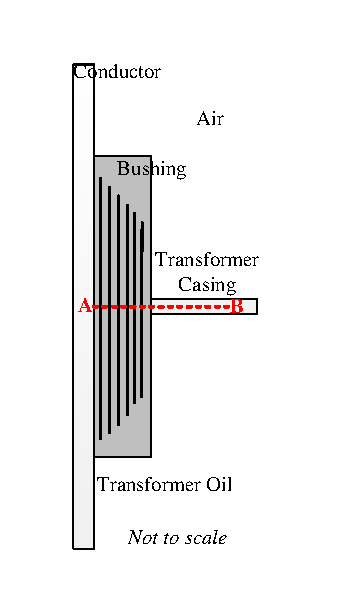
\includegraphics[width = 0.16\textwidth]{./Figures/CutLocation_Mid.pdf} 
	%\caption{Normal Electric Field (V/m) for the No-Grading Model}
	\label{Figure:Cut_NoFoil_Mid}
   } 
\subfigure[The No Foils Model Fails PD Criteria]{
    \includegraphics[width = 0.55\textwidth]{./Figures/MatlabFigs/No_Foil_Mid.eps} 
	%\caption{Normal Electric Field (V/m) for the No-Grading Model}
	\label{Figure:NoFoilsFail}
   }
\caption{The Normal Electric Field in the No Foils Model}
\label{Figure:Radial_No_Foils_Fails}
\end{figure}

\begin{figure}[!h]
  \centering
\subfigure[Location of Cut Plane(s)]{
    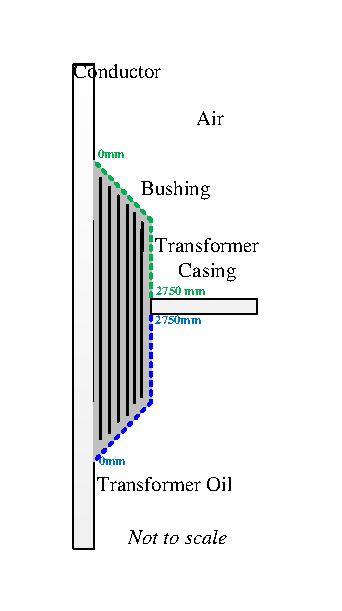
\includegraphics[width = 0.18\textwidth]{./Figures/CutLocation_Axial.pdf} 
	%\caption{Normal Electric Field (V/m) for the No-Grading Model}
	\label{Figure:Cut_NoFoil_Axial}
   } 
\subfigure[The Axial Electric field along the bushing surface]{
    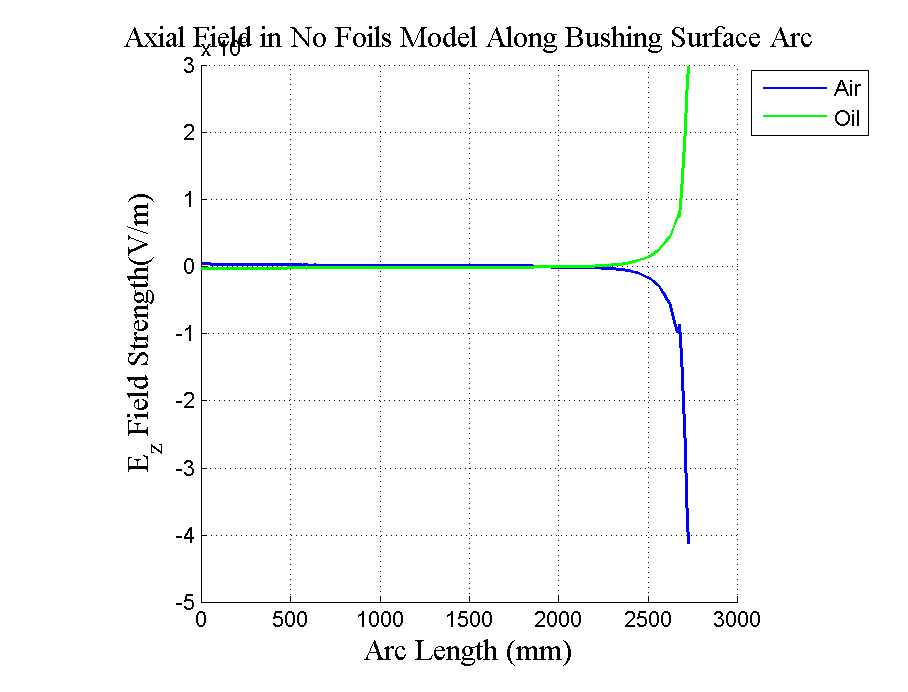
\includegraphics[width = 0.5\textwidth]{./Figures/MatlabFigs/No_Foil_Surface_AxialField.eps} 
	%\caption{Normal Electric Field (V/m) for the No-Grading Model}
	\label{Figure:Nofoilsaxialfield}
   }
\caption{Axial electric field along the surface of the bushing}
\label{Figure:Nofoilsaxialfieldwhole}
\end{figure}

This is best illustrated with figure \ref{Figure:NoFoilsFail}, not only are the fields present at the interface to the flange well in excess of the PD inception voltage, the location of these high electric fields also mean flashover is a serious risk due to the lack of shaping of the axial electric field distribution. A result of such localised electric stress is that because the field is greater than the PD inception voltage the voids will generate exponentially more discharges, leading to faster ageing and a much higher chance of breakdown. The solution, assuming keeping voltage constant, would be to increase the bushing height and width. 


\subsection{No Grading}
%BH
%fig 6.11b, 6.11c
%same graph as 7.1 but for no grading
%done but need to make .fig into pdf then add to latex (help needed)
The proposal to study a model of condenser bushing without any thought to grading exposes the fundamentals to grading design. Figure \ref{Figure:NoGrad1D} shows that, for the most part the electric field is below the PD inception voltage, at least at the central interface. However looking at figures \ref{Figure:No_Grading_Field_CloseMid} and \ref{Figure:No_Grading_Field_CloseTip} show that the foil placement did not effectively shape the field at the bushing interface at the tips.  Beyond analysing the concentrations of electric field it is important to note that the distribution is non-linear; in comparison to the ideal goal of a linear drop of field across the capacitors \citep{kuffel2000high}. The placement of the outermost foil serves as a location of high field density and although located far from the flange itself it would likely be a source of both PDs and corona discharges. 

\begin{figure}[!h]
  \centering
\subfigure[Location of Cut Plane]{
    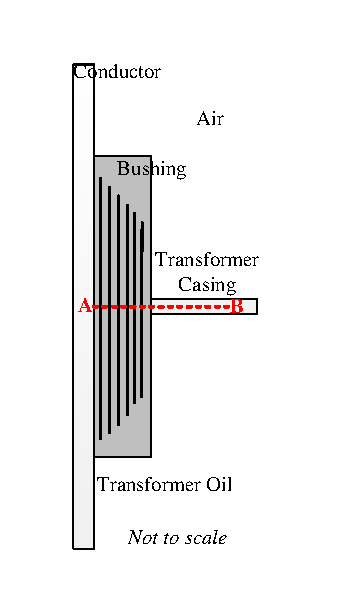
\includegraphics[width = 0.16\textwidth]{./Figures/CutLocation_Mid.pdf} 
	%\caption{Normal Electric Field (V/m) for the No-Grading Model}
	\label{Figure:Cut_No_Grad_Mid}
   } 
\subfigure[The No Grading Model Fails PD Criteria]{
    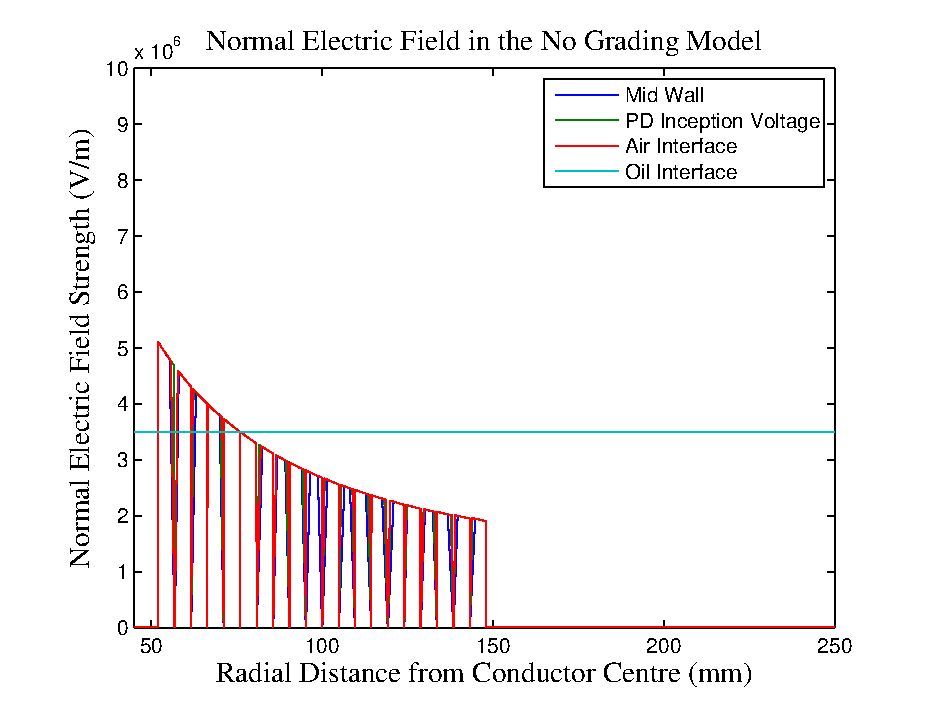
\includegraphics[width = 0.55\textwidth]{./Figures/MatlabFigs/NormEfieldinnograding.eps} 
	%\caption{Normal Electric Field (V/m) for the No-Grading Model}
	\label{Figure:NoGrad1D}
   }
\caption{The Normal Electric Field in the No Grading Model}
\label{Figure:No_Grad_Failing}
\end{figure}

% want a plot of the tips?

\begin{figure}[!h]
  \centering
\subfigure[Location of Cut Plane(s)]{
    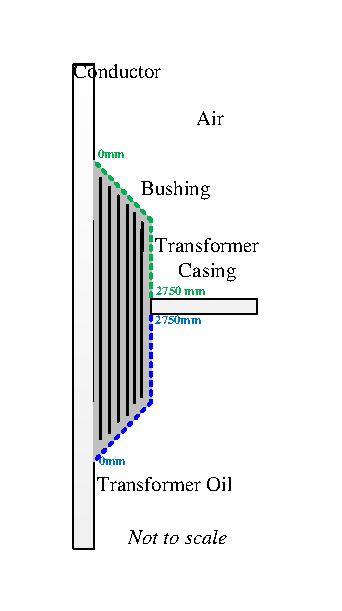
\includegraphics[width = 0.18\textwidth]{./Figures/CutLocation_Axial.pdf} 
	%\caption{Normal Electric Field (V/m) for the No-Grading Model}
	\label{Figure:Cut_NoGrad_Axial}
   } 
\subfigure[The Axial Electric field along the bushing surface for no-grading model]{
    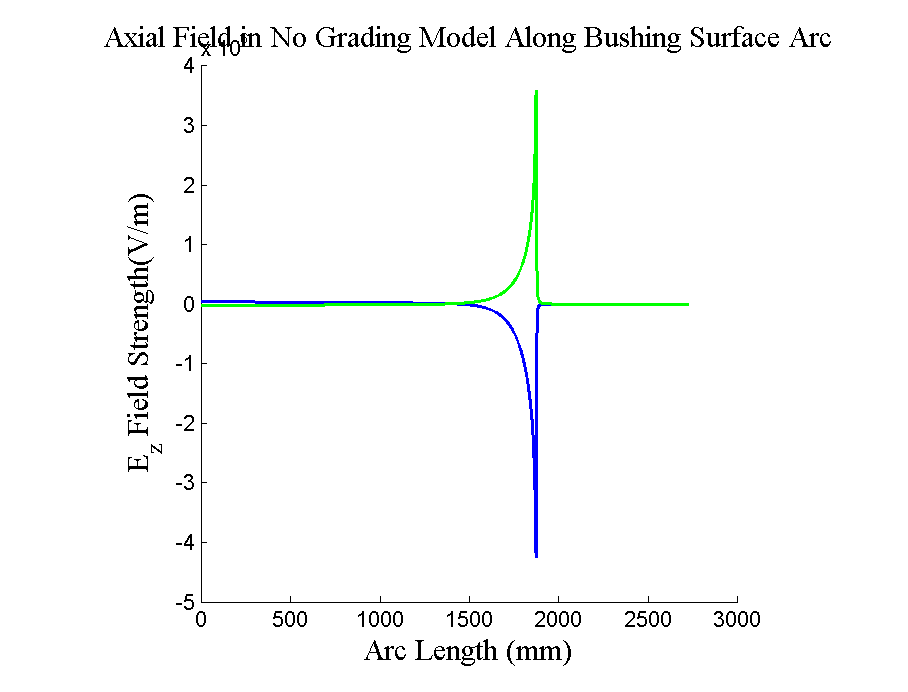
\includegraphics[width = 0.5\textwidth]{./Figures/MatlabFigs/No_Grading_Surface_AxialField.eps} 
	%\caption{Normal Electric Field (V/m) for the No-Grading Model}
	\label{Figure:Nogradaxialfield}
   }
\caption{Axial electric field along the surface of the bushing}
\label{Figure:Nogradaxialfieldwhole}
\end{figure}

%\begin{figure}[!h]
%	\centering
%	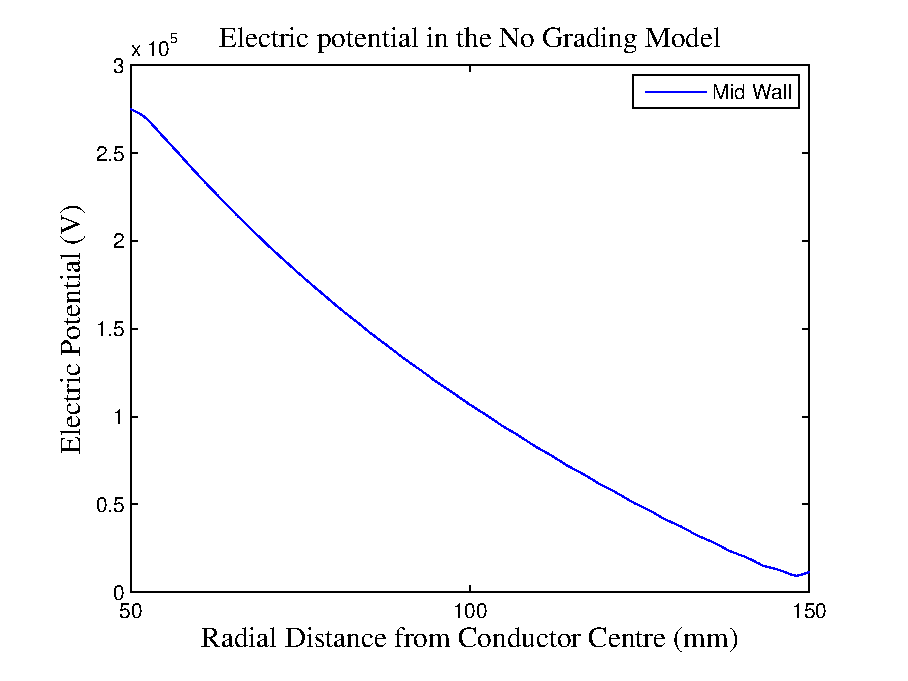
\includegraphics[width= 0.5\textwidth]{./Figures/MatlabFigs/No_Grading_Electric_Potential.eps}
%	\caption{The Electric potential across the midwall}
%	\label{Figure:Nofoilsaxialfield}
%	\end{figure}

\begin{figure}[!h]
  \centering
\subfigure[Location of Cut Plane]{
    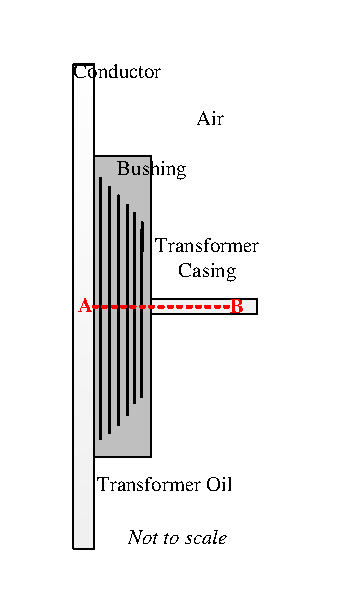
\includegraphics[width = 0.16\textwidth]{./Figures/CutLocation_Mid2.pdf} 
	%\caption{Normal Electric Field (V/m) for the No-Grading Model}
	\label{Figure:Cut_No_Grad_Mid}
   } 
\subfigure[The Electric potential across the midwall]{
    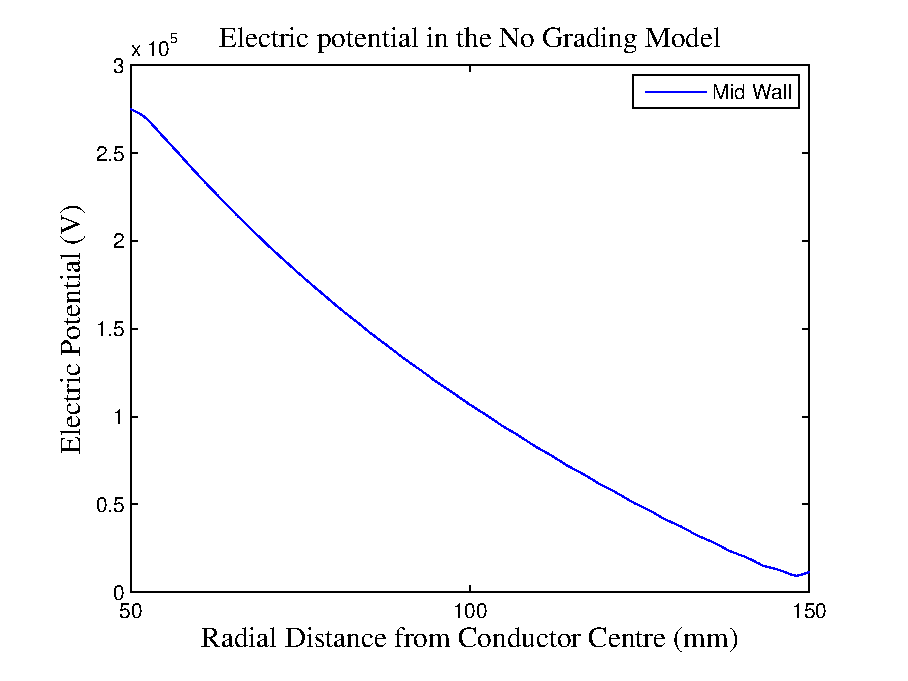
\includegraphics[width = 0.55\textwidth]{./Figures/MatlabFigs/No_Grading_Electric_Potential.eps} 
	%\caption{Normal Electric Field (V/m) for the No-Grading Model}
	\label{figure:nogradpotentialmid}
   }
\caption{The electric potential within the no grading model}
\label{Figure:No_Grad_Failing_potential}
\end{figure}


\subsection{Comparison of Axial and Radial Grading Solutions}
The design of both types of capacitive grading method were discussed in the previous sections. The difference in performance of the types in general is the radial grading will improve the intensity of the radial electric field and the axial grading will improve the intensity of the axial electric field. By improvement of intensity of electric field, this means the electric field according to the type of grading method is evenly distributed in a particular direction. Choosing the right design for different application is essential as this will reduce the chances of various types of electrical breakdown and hence the bushing design would be more durable.

There are two components of electric field cause different problems. The radial electric field is mainly responsible to the breakdown of insulating material, for example, electrical breakdown between foils. On the other hand, the axial electric field is mainly responsible to the surface discharges along the boundary of the insulation, for example, corona discharge to the surrounding.

\subsubsection{Radial Electric Field}
The maximum intensity of the radial electric field for the radial design is expected to be lower than the maximum of the axial design. This means the radial grading design would perform better to suppress the intensity of radial electric field. The radial electric field across the radial direction of both axial and radial grading designs are shown in figure \ref{figure:rfield}.

\begin{figure}[!h]
  \centering
\subfigure[Location of Cut Plane]{
    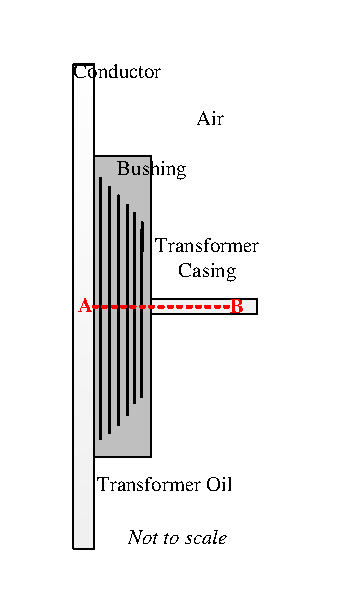
\includegraphics[width = 0.16\textwidth]{./Figures/CutLocation_Mid2.pdf} 
	%\caption{Normal Electric Field (V/m) for the No-Grading Model}
	\label{Figure:Cut_No_Grad_Mid}
   } 
\subfigure[Radial electric field across the mid-point of the two designs of bushing.]{
    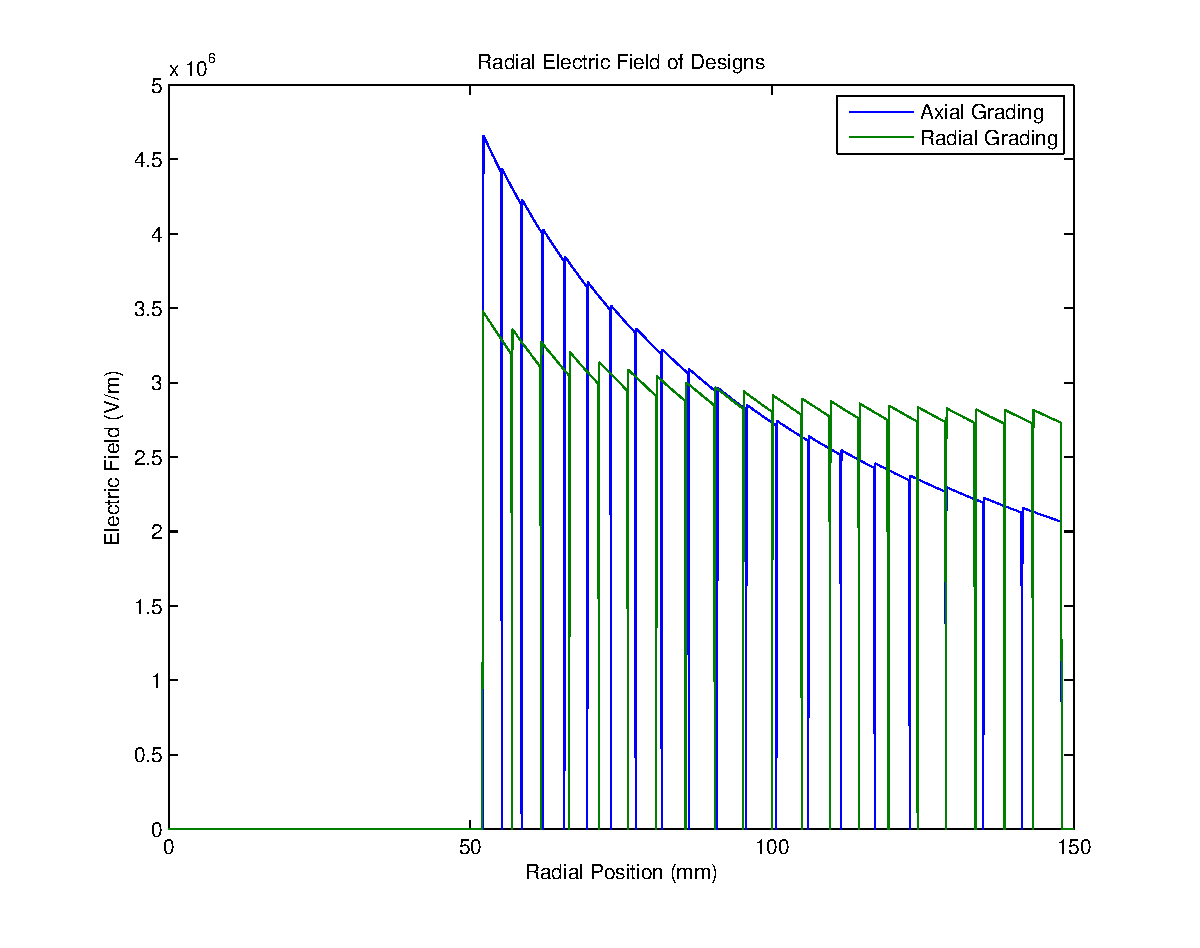
\includegraphics[width = 0.55\textwidth]{R-field.eps} 
	%\caption{Normal Electric Field (V/m) for the No-Grading Model}
	\label{figure:rfield}
   }
\caption{The Normal Electric Field in the No Grading Model}
\label{Figure:No_Grad_Failing}
\end{figure}


\begin{figure}[!h]
\centering
\includegraphics[width=\textwidth]{ConstantAxialField.eps}
\caption{2D surface plot showing the distribution of electric field from mid-point to the air end of bushing}
\label{figure:constantfield}
\end{figure}
The result clearly shows the peak value of electric field for the axial design ($\approx 4.5 \times 10^3 kVm^{-1}$) is greater than the peak value of electric field for the radial design ($\approx 3.5 \times 10^3 kVm^{-1}$). Also, from the figure \ref{figure:rfield}, the radial electric field of the radial grading design is more evenly distributed. This is the effect of grading, hence similar effect should be seen in the axial electric for axial grading design. The electric field distribution across any perpendicular cut lines to the foils would result in almost identical results, because the foils behave similar to capacitors in series. Electric field being constant across a capacitor and this is true across any two neighbouring foils. Figure \ref{figure:constantfield} shows the electric field with in foils from mid-point to the tips and very constant electric field is seen.



\subsubsection{Axial Electric Field}
The axial component of electric field is responsible for the surface discharges along the surface of the bushing design. Axial component of the field contributes to these surfaces, because the axial electric field at the edges of the foil are the most intense. Figure \ref{figure:afield} shows the magnitude of electric field at each foil edge. 

\begin{figure}[!h]
\centering
\subfigure[Air side axial electric field]{
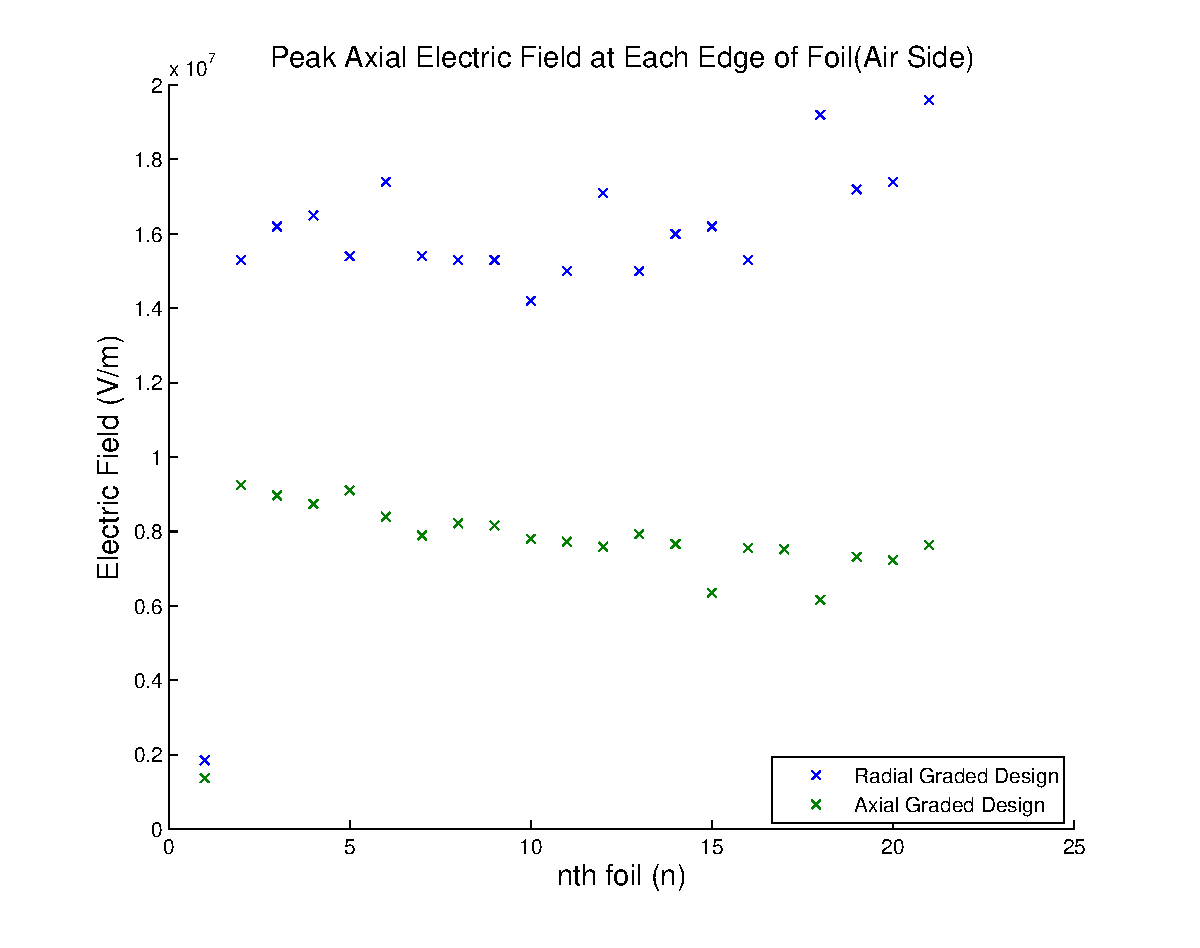
\includegraphics[width = 0.7\textwidth]{A-fieldA.eps}
\label{figure:afielda}
}
\subfigure[Oil side axial electric field]{
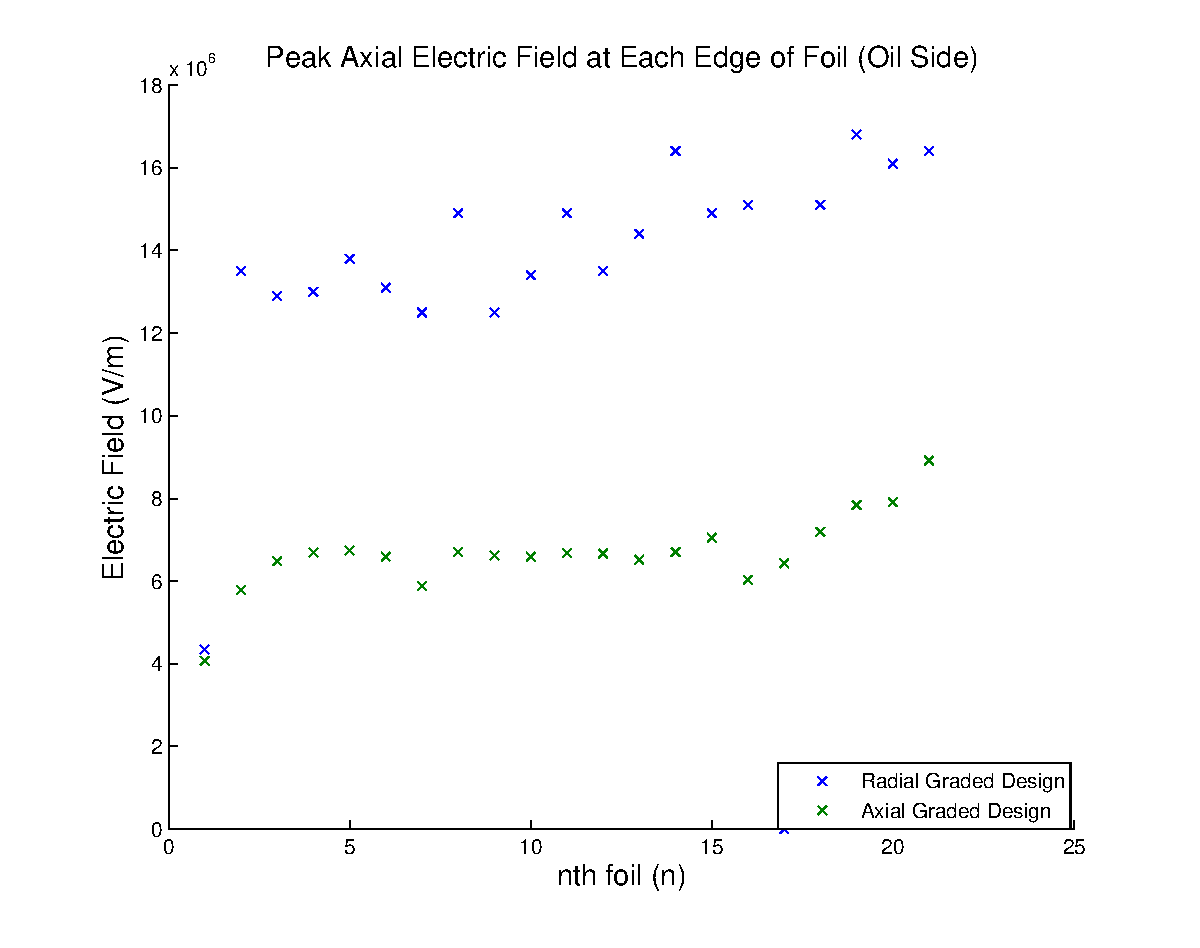
\includegraphics[width = 0.7\textwidth]{A-fieldO.eps}
\label{figure:afieldo}
}
\caption{Electric field at the edge of each foil.}
\label{figure:afield}
\end{figure}

The result shows the radial design has a lower peak value of electric field at these edges of foil. However, this is not an expected result, because axial grading in theory shapes the surface of the insulation better to avoid intensifying of electric field at these edges. Also, a clearer maximum peak of electric field at should be seen at the outermost foil of the radial graded design due to the sharp turn in the shape of the bushing design. Although the result shows a maximum peak at the last outermost foil, it is not significant and it is below the maximum value of electric field for the axial graded design. Although the radial graded design has lower maximum electric field than the axial graded design, the electric field generally is much greater than the partial discharge inception voltage for oil-impregnated paper insulation. This will result in partial discharge.

However, The points which are taken in to consideration are the highest values of electric field locally which drops off rapidly moving away from the point. While the sum of these points is approximately 0.03\% of the volume of the overall bushing design, hence, this can be consider as an affordable problem in the bushing design. Also, in the model, all the foils are considered to terminate with a $90^\circ$ bend. In reality, designs may use various various techniques to suppress the effect of this bend. Some design uses semi-conducting material at the ends of the foil. %citation

\subsubsection{Surface Flashover}
%talk about the addition of shedding in completeness. Limitations of current model without shedding -> primarily some extra shaping of fields. The effect of grounding the outermost capacitor.
%===============================================
Surface flashover is the partial discharge along the surface of the insulation, this is cause by a intense electric field. The parameter which takes into account of surface flashover is the creepage distance as mention previously. The typical value for calculating the creepage distance is 35mm/kV %need a reference for this prob%
and for more polluted environment, a higher value of creepage distance might be considered.

In bushing designs, the creepage distance is increased by the addition of a shed around the bushing. These shed designs increase the creepage distance of insulation designs by increasing the surface length.  Designs of shed can have varying ratios between creepage distance to axial length \cite{shed}, designs for more polluted environment have bigger ratios.

According to the typical value to calculate the creepage distance, for a 275kV design, the creepage distance required is 9625mm. Where the designs of bushing in this report has axial length of approximately 3m, the ratio of minimum nominal creepage distance to axial length required is 3.2:1.

These shed provides a greater creepage distance to reduce the chance of surface flashover, however, they have little affect on the electric field of the bushing. Hence, addition of shed does not reduce corona discharge. 

\subsection{Design Improvements}
The high electric field at the tips of the foils has been identified as a cause for concern.
The field strength at this point exceeds the PD inception voltage by double in the axial design, and around four times in the radial design.
It is therefore necessary to improve the base design.

The first aspect to consider is the accuracy and relevance of the COMSOL model.
The very thin foils are modelled as perfect rectangles with sharp $90^{o}$ corners.
This approximation was made to make the geometry of the model simple for input to COMSOL.
Sharp corners cause areas of exceedingly high field strengths. 
A refined model was required, to confirm that the unrealistic sharp corners on the foils were not causing the exceedingly high field strengths.

The radial model was taken forward, since it already passes the radial field criteria.
If a way to reduce the field at the foil tips could be found, the radial design would pass all criteria.
The end of each of the foils was filleted, so that the ends formed a semi-circle.
While this is still not the optimum design for an electrode, it is certainly an improvement over the sharp angles.

\begin{figure}[!h]
\centering
\subfigure[Curved Foil Tips]{
\includegraphics[width = 0.45\textwidth]{./Figures/Simulations/Improvements/Curved.eps}
\label{figure:Curved}
}
\subfigure[Angled Foil Tips]{
\includegraphics[width = 0.45\textwidth]{./Figures/Simulations/Improvements/Old.eps}
\label{figure:Angled}
}
\caption{Normal Electric Field at the Tips Improvement}
\label{figure:curvedcompare}
\end{figure}

The curved foil tip is clearly visible in figure \ref{figure:Curved}.
There is an improvement, the curved design has a slightly smaller area of field strengths higher than the threshold.
However, it has not solved the issue completely.
Further design modifications are required.

Literature on bushing design refer to the high field at the tips problem \cite{kuffel2000high}.
One possible solution commonly suggested is to coat the tip of the foil in a semiconductor.
\inote{BH can you add a little bit here about the semiconductor thing - references and why would it help?}

This has been modelled in COMSOL by adding a square to the edge of the foil $0.1mm$ in dimension. 
The outer edges of the square are filleted to a curve in the same way the tips were previously.
These squares were allocated the relative permittivity of $\epsilon_r = 11.7$, which is the permittivity of silicon.
The actual manufacture processes are not in the scope of this report, and different semiconductors may be used in industry.
However, adding this to the COMSOL will at least prove the concept.

\begin{figure}[!h]
\centering
\subfigure[Semiconductor Foil Tips]{
\includegraphics[width = 0.45\textwidth]{./Figures/Simulations/Improvements/Semi.eps}
\label{figure:Semi}
}
\subfigure[Angled Foil Tips]{
\includegraphics[width = 0.45\textwidth]{./Figures/Simulations/Improvements/Old.eps}
\label{figure:Angled2}
}
\caption{Normal Electric Field at the Tips Improvement}
\label{figure:semicompare}
\end{figure}

The semiconductor block with curved edges can be seen in figure \ref{figure:Semi}.
It is shown alongside the original angled design for comparison in figure \ref{figure:Angled2}.
Once again, there is a subtle improvement in the area exposed to very high field concentrations.
However, it remains well above the $4.5kV/mm$ threshold value.

The normal electric field values have been extracted and plotted in figure \ref{figure:scattercomp} to enable a more direct, quantitative comparison.
It is clear that the radial semiconductor tipped model has reduced the field strength by almost half, and is nearly at the same level as the axial field design.
The curved foil design is an improvement, but the semiconductor design has a significant impact on the field distribution.

\begin{figure}[!h]
\centering
\includegraphics[width=0.8\textwidth]{./Figures/Simulations/Improvements/RadialScatter.eps}
\caption{Scatter showing the normal electric field at the tips of each foil in the axial, radial, radial curved and radial semiconductor models.}
\label{figure:scattercomp}
\end{figure}


\subsection{Choice of Design}
From the results shown in the previous sections, the graph of variation in radial electric field shows the peak radial electric field for the axial graded design, the limit of 4.5kV/mm is just exceeded. While the radial graded design have radial electric field below the limit. However, the axial electric field in both design exceeds the limit by a few times in some places. More importantly, the axial electric field for the radial graded design is in general approximately twice as much as the axial graded design. Hence, the results show the radial design suppresses more in radial electric field, while the axial electric field is suppressed more in the axial graded design as expected. The choice of which design to use would depend on the effect of the axial and the radial electric field. Whether the doubling effect in the axial electric field would cause a bigger problem or would the excessive radial electric field cause a bigger problem. According to the weakness for bushing designs, the axial electric field usually cause more problems as the breakdown within foil would require a higher electric field than surface discharge along the boundary layer. So, the axial graded design would be used when taken all these factors into consideration.

\section{Conclusions}
All of the different designing method in bushing design are about suppressing the intensity of electric field throughout the system as these intensification of electric field causes the various types of breakdown. Focusing on high voltage AC bushing designs, capacitive grading methods are used typically used to control the electric field distribution along the desired boundaries. This control of electric field based on the concept of constant electric field %here
By controlling the electric field, evenly distributed electric field can be achieved. Also, depending on the type of grading method used suppression of peak in the specific component of electric field is achieved

%regarding area of interest of tips of foils a suggestion in (Graham?) was to line the capacitors with semiconductor material to more evenly spread out the field distribution.
